Testing of AJFS was completed on a small cluster of 8 nodes. Each node in the
cluster was a virtual machine with two cores on a 2.8GHz Intel Xeon CPU. The
systems run Ubuntu 12.04.2 LTS with Linux kernel 3.2.0-39. The nodes each have
2GB of RAM, and share an NFS mounted set of home directories.  Tests were run in
userspace running over NFS. No client-side caching was disabled.

The systems supported FUSE 2.8.6 and Apache Thrift 0.9.0. AJFS was evaluated for
both consistency and performance.

\subsection{Consistency}
The main design goal of AJFS requires file consistency across multiple servers,
and as a result, evaluation of safety and file consistency is the most important
measure of whether AJFS has achieved its objectives.

What follows are the descriptions of a few simple tests and use cases that,
among others, suggest consistency despite a variety of perturbations. 

\subsubsection{Server crash and rejoin}

In distributed system, it's common that a server crashes. We need to guarantee
that when a server is down, data that changes while a server is offline is not
lost, and when the dead server comes back online, the data is synchronized.

% The design of AJFS supports server rejoins. Since it's running based on the
% local backup, client can access the file locally without issue, just like
% Coda~\cite{KS92} does.  The only problem is when the server is down, client
% cannot access the mount point, because fuse server is also down. Instead,
% client should access the local backup. When the server rejoins, it will
% automatiaclly rsync with remote repositories and sync up the local files with
% remote replicas.

Specifically, we tested the following scenario on AJFS:

\begin{enumerate}
    \item AJFS is running with three servers $A$, $B$ and $C$; we kill server
        $C$; client $a$ on server $A$ creates file $x$; we then restart server
        $C$.
    \item AJFS is running with three servers $A$, $B$ and $C$; client $a$
        on server $A$ creates file $x$ and starts writing to it. While writing, we kill server
        $C$. Client $a$ then completes $x$ and we restart server $C$.
\end{enumerate}

In both cases, we were able to successfully retrieve a complete and accurate
file $x$ on server $C$.

The test shows that AJFS is robust against a common occurance: a server dying
while other operations continue. Consistency is still maintained across systems.

\subsubsection{Write protection}

Many distributed systems support mulitple simultaneous writes.
TreadMarks~\cite{treadmarks} supports multiple writers; Bayou~\cite{bayou} askes
each writer to provide dependency check and merge procedures.
However, AJFS choosees to not permit this functionality to avoid the possibility
of conflicts and to maintain simplicity.

A possible solution to support multiple simultaneous writers in AJFS is copy on
write. The write operation only writes to the local copy, and when the file is
closed, the modifications is propagated to the replicas. We do not use this
mechanism because the merge procedure on server the side may be complicated.
Another solution to this issue is to keep different conflict versions of a
single file. 

Instead, we chose locks and only allow one writer to a file at one time, which
is simple and easier to maintain correctness. Given our non-collaborative
expected use cases, this is also completely reasonable.

We tested many cases, drawing special attention to the following cases on AJFS
with two servers $A$ and $B$:
\begin{enumerate}
\item Client $a$ on server $A$ writes to file $x$; at the same time client $b$ on
sever $B$ opens file $x$ for read.
\item Client $a$ on server $A$ writes to file $x$; at the same time client $b$ on
sever $B$ opens file $x$ for write.
\item Client $a$ on server $A$ reads file $x$; at the same time client $b$ on
    sever $B$ tries to delete parent folders of file $x$.
\end{enumerate}

On AJFS, all the test cases work as expected; For test case 1, client $b$ can
not open the file for read, because we only allow one writer OR multiple
readers. For test case 2, the request from client $b$ is similarly declined. For
test case 3, AJFS denies the operations, specifying that there are no locks
available. These results suggest that AJFS maintains file consistency in the
presence of multiple interacting clients.

\subsubsection{Rapid Writing and Hash Testing}

In order to develop some faith in Thrift and the approach taken by AJFS, we
tested AJFS under a series of high-throughput "nightmare" scenarios. Tested
across 8 nodes, we performed a series of randomized file writes originating from
all servers. To verify correctness, MD5 hashes were calculated for all generated
files across all of the servers. The hashes were then cross-checked across the
servers to ensure that all nodes had identical files.

This ended up being a great debugging test, but ultimately successfully handled
dozens of writes up to 1 GB each without any data loss.

\subsection{Performance}

Performance is \textbf{not} the key motivation of AJFS. Using AJFS to sync up
big files is not efficient as AJFS needs to propagate the data to
all the nodes during the initial write. However, in order to understand how to
improve AJFS, it is useful to understand its current limitations.

Figure~\ref{fig:writeperf} shows the average performance of a \texttt{write()}
under AJFS with a varying number of nodes, as compared with a basic example
using FUSE, and the base file system performance. These values are measured
using the Unix command \texttt{dd}. The results remain consistent regardless of
how much data is written with a single \texttt{write()} call.

There is a clear trend that with the number of AJFS nodes increasing, the write
bandwidth of AJFS decreases. This is because although AJFS uses asynchronous
write propagation in that it does not wait for the response from remote nodes'
operations, it still must transfer the data to other hosts synchronously.
As more nodes means more nodes to transfer to (as each transfer is unicast), the
performance degrades with the number of nodes increasing. 

Figure~\ref{fig:readperf} shows performance of a \texttt{read()} operation under
AJFS with a varying number of nodes. It is constant with respect to the number
of nodes, and is also close to the base FUSE read performance.
This is because AJFS handles \texttt{read()} operations locally and does not
propagate non-modifying requests to other servers.

In both graphs, there is a significant difference in performance between the
local file system and FUSE/AJFS. The version of FUSE used on these systems
clearly adds significant overhead, but this overhead resides in FUSE rather than
in AJFS.

It is worth noting that in the AJFS \texttt{read()} throughput graph, the tests
are fairly obviously benefitting from a file buffer cache. Rather attempt to
measure performance in an artificial-use scenario, we opted to allow the
caching. We believe these speeds more accuraely reflect real-life usage
patterns. FUSE does not add any additional caching, and instead we rely on the
caching of the underlying file database.


\begin{figure}[Ht]
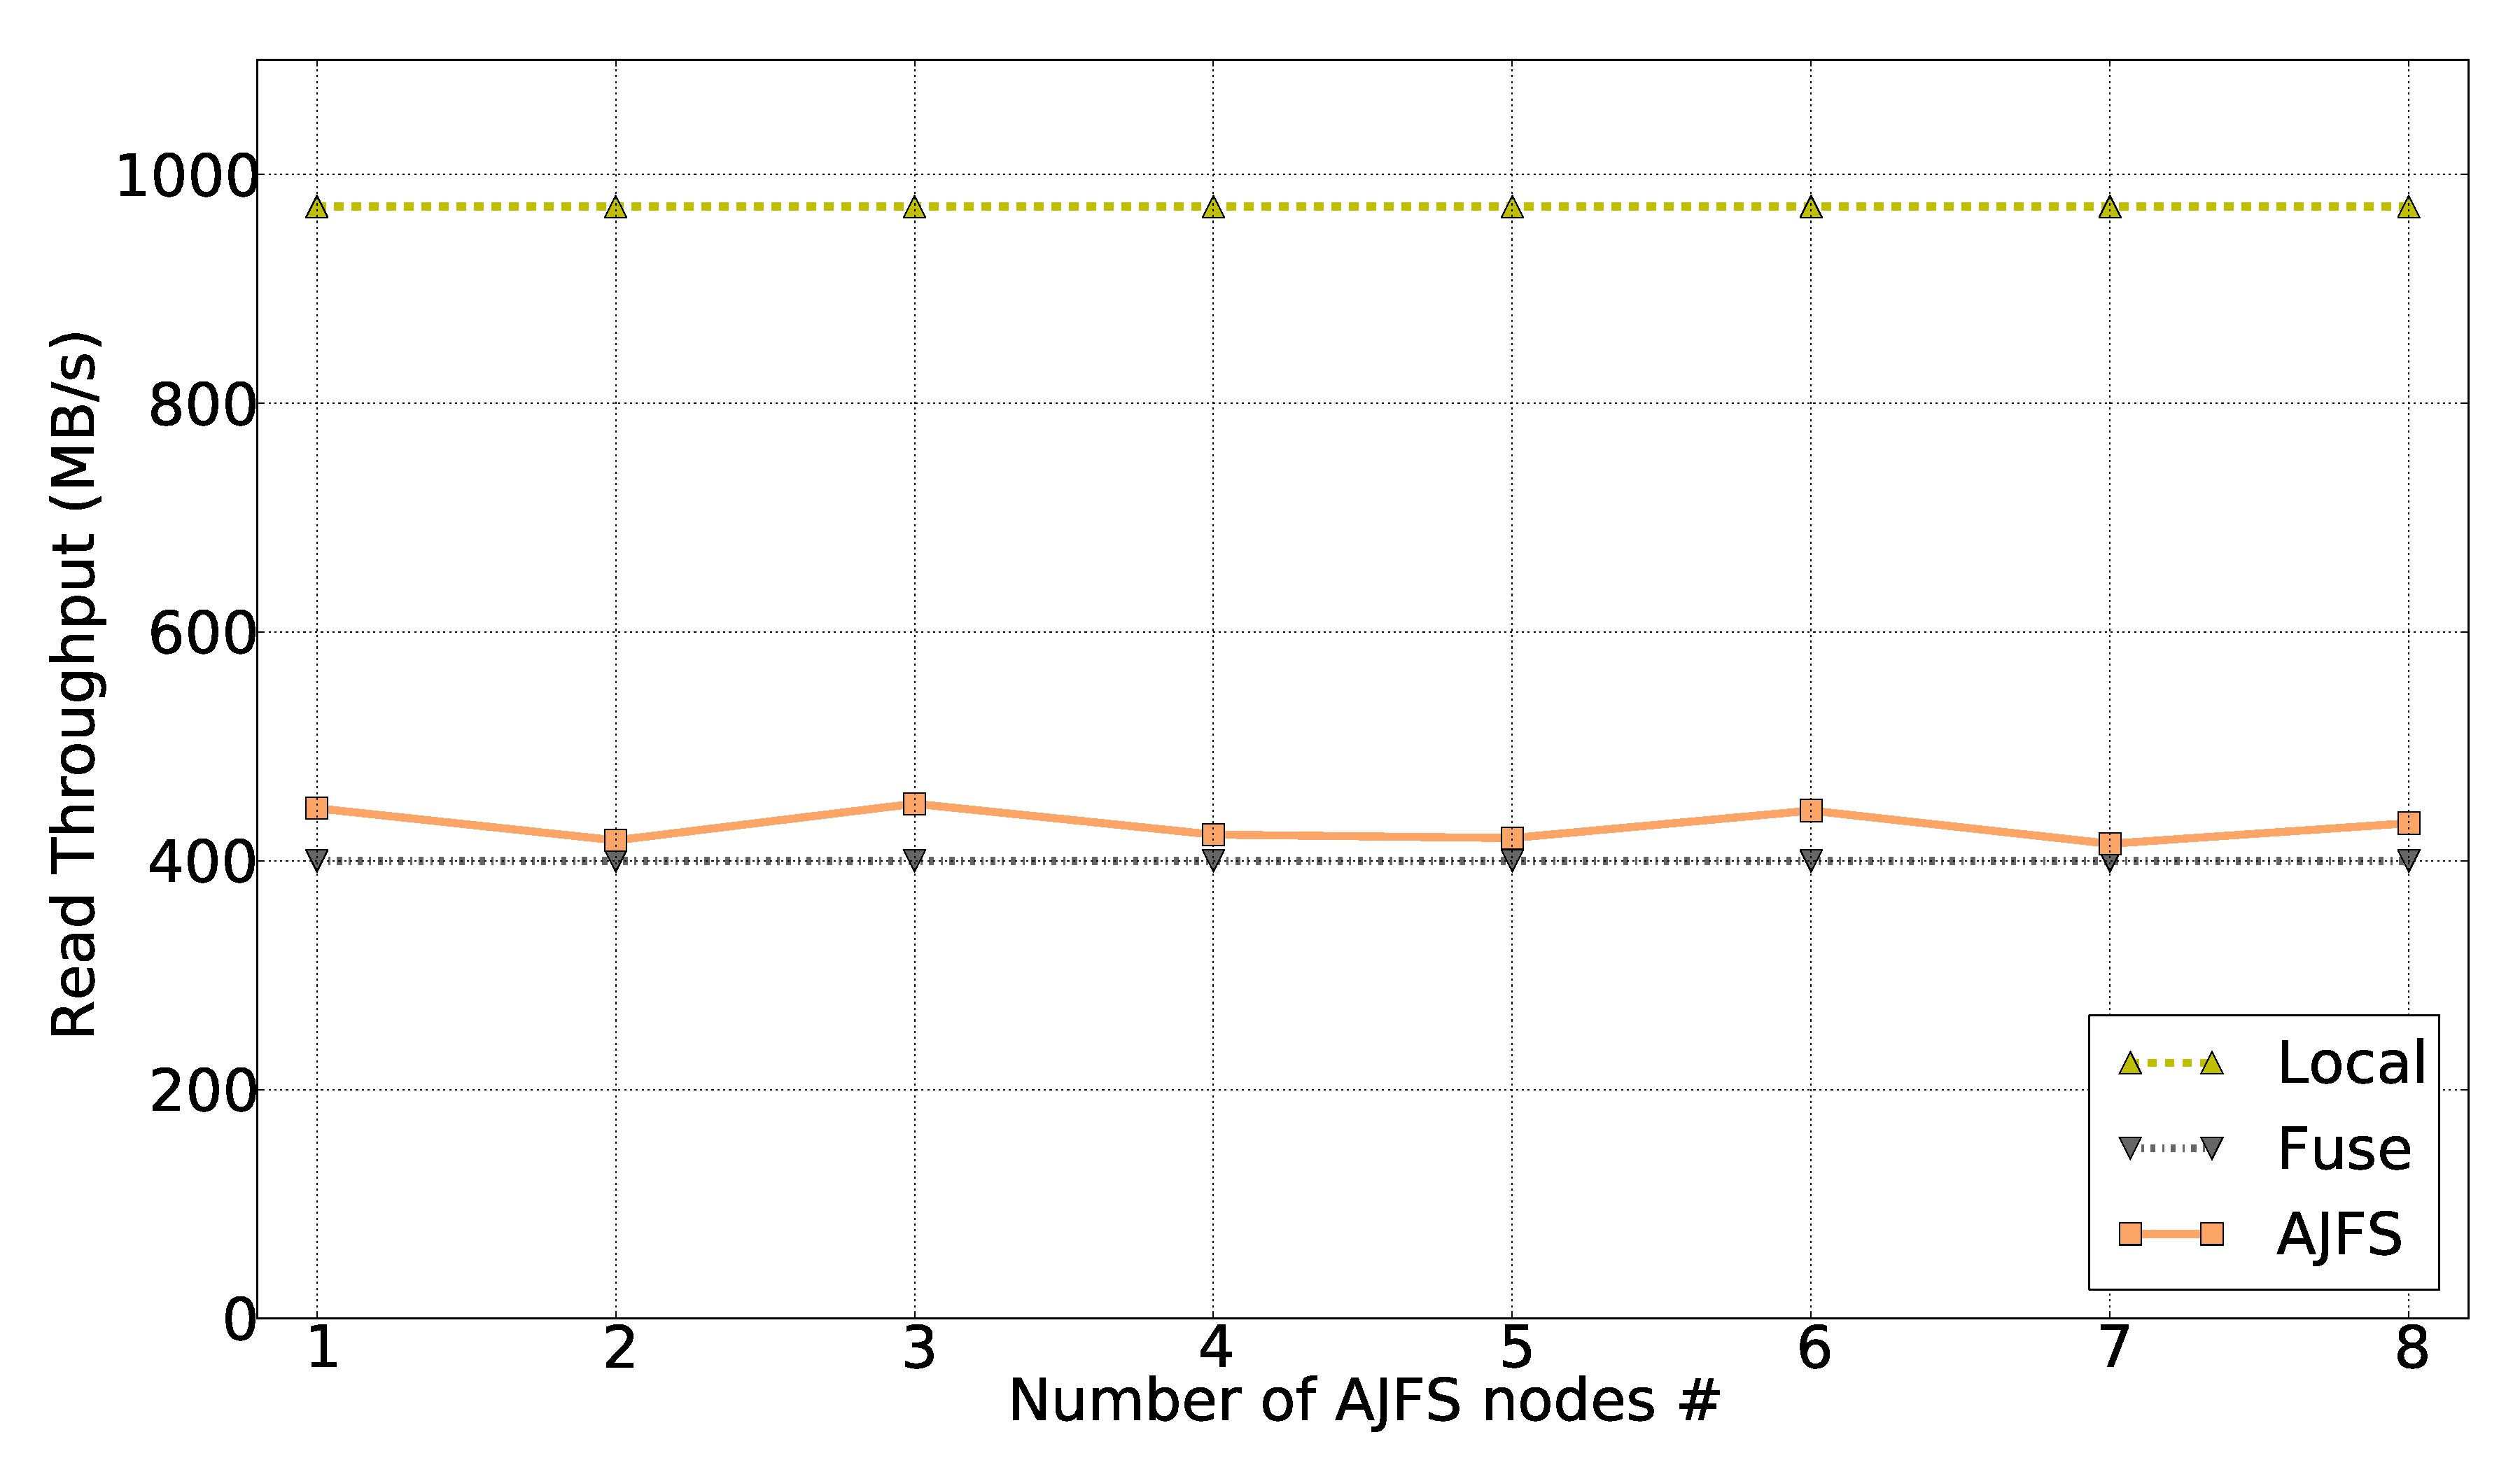
\includegraphics[width=\linewidth]{readperf.pdf}
\caption{AJFS Read Performance}
\label{fig:readperf}
\vspace{-5mm}
\end{figure}

\begin{figure}[Ht]
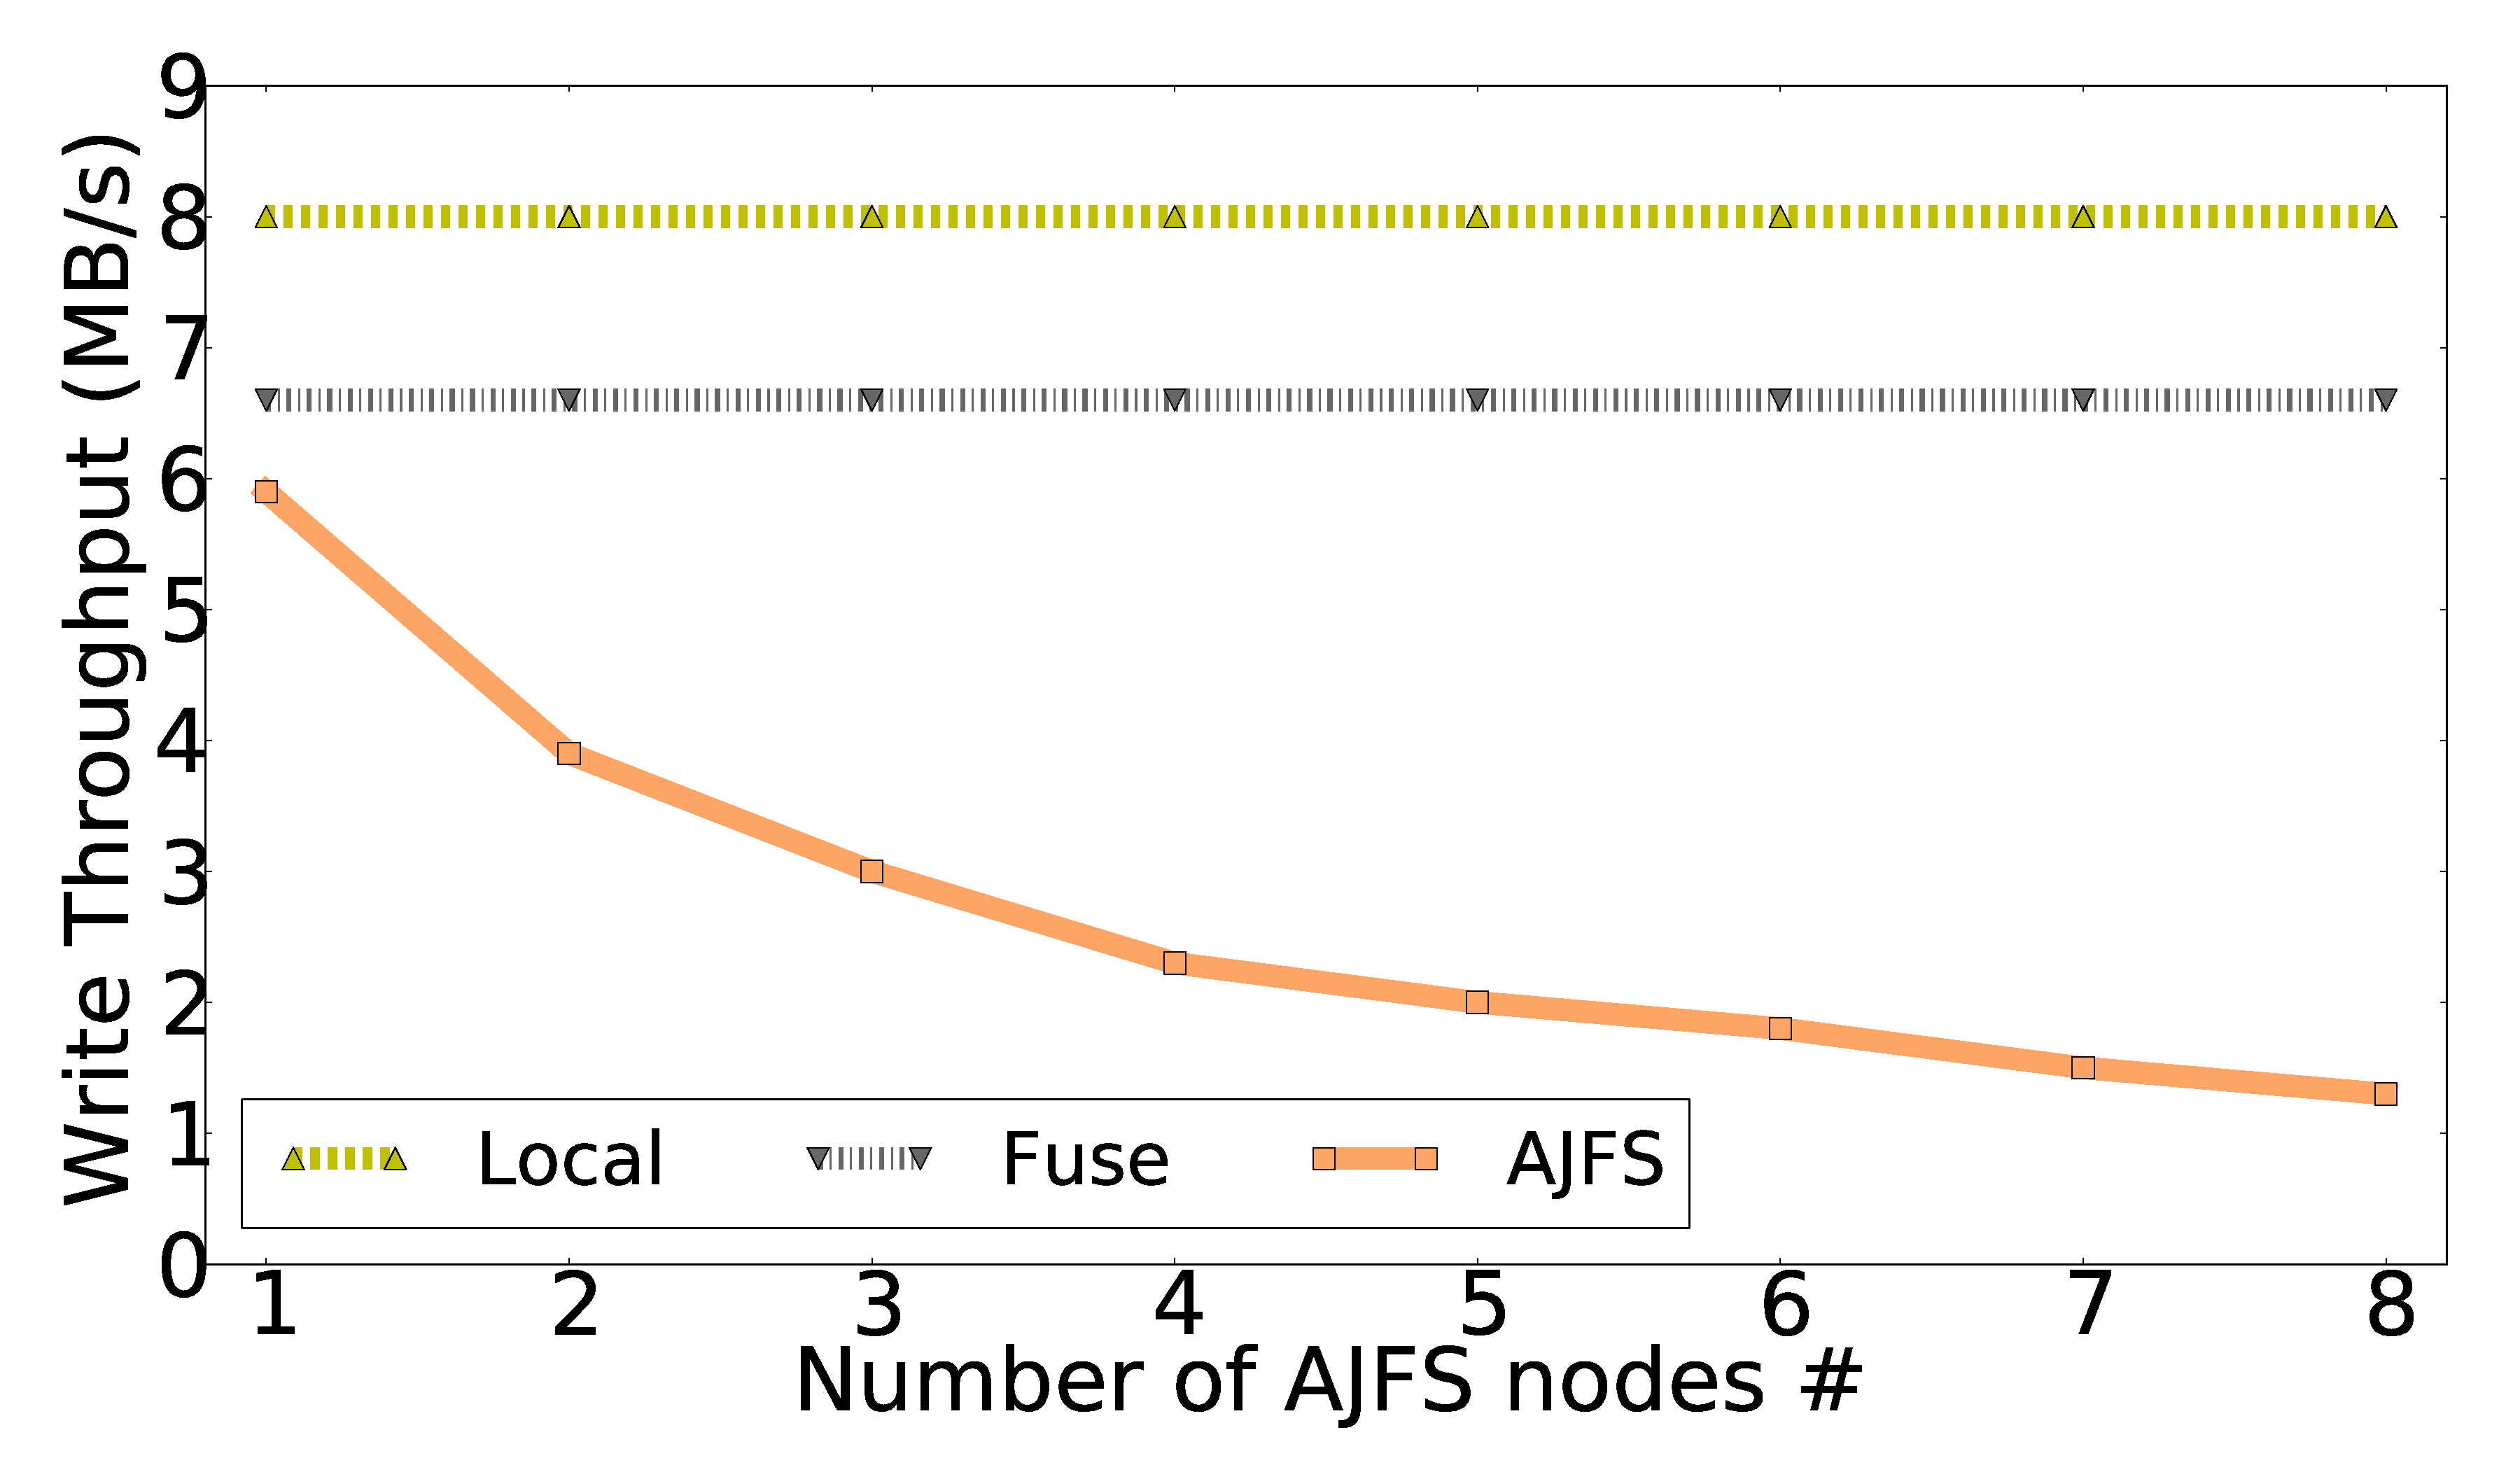
\includegraphics[width=\linewidth]{writeperf.pdf}
\caption{AJFS Write Performance}
\label{fig:writeperf}
\vspace{-5mm}
\end{figure}

\subsection{FS Benchmarks with Bonnie++}

We further do some limited testing of performance of AJFS with Bonnie++
\cite{bonnie++}. Bonnie++ is a benchmarking tool designed to test file system
performance by doing "database type" file access. It tests file creation,
reading, writing and deleting files in a variety of patterns. For the most part,
Bonnie++ tests are more information than is needed for testing AJFS, as
performance of AJFS is so closely related to the performance of the underlying
system.

Tables~\ref{tab:bonnie-8n}, \ref{tab:bonnie-1n},
\ref{tab:bonnie-fusexmp_fh} and \ref{tab:bonnie-nfs} present the results
from running Bonnie++ with a total file size of 4GB under AJFS with eight nodes,
AJFS with one node, a simple FUSE wrapper and the base file system. All systems
use NFS to a remote 'black box' file server on the backend.

For the most part, these results%
\endnote{A full explanation of the Bonnie++ output is beyond the scope of this
writeup, but more information is available at \url{http://www.coker.com.au/bonnie++/readme.html}
}
are consistent with the \texttt{dd} tests, and further show that writing
operations all suffer relatively uniformly, while reading operations are
relatively lightweight.

\begin{table}[Ht]
\centering
\begin{tabular}{| c | c | c | c | c | c |}
\hline
\multicolumn{6}{|c|}{\bf Sequential Output}\\
\hline
\multicolumn{2}{|c|}{Per Char} &
\multicolumn{2}{c|}{Block} &
\multicolumn{2}{c|}{Rewrite} \\
\hline
K/sec & \%CP & K/sec & \%CP & K/sec & \%CP \\
\hline
 1500 & 3 & 1567 & 0 & 1481 & 0 \\
\hline

\multicolumn{4}{|c|}{\bf Sequential Input} & \multicolumn{2}{c|}{\bf Random}\\
\hline
\multicolumn{2}{|c|}{Per Char} &
\multicolumn{2}{c|}{Block} &
\multicolumn{2}{c|}{Seeks} \\
\hline
K/sec & \%CP & K/sec & \%CP & /sec & \%CP \\
\hline
 31354 & 63 & 41290 & 5 & 139.8 & 0 \\
\hline

\multicolumn{6}{|c|}{\bf Sequential Create}\\
\hline
\multicolumn{2}{|c|}{Create} &
\multicolumn{2}{c|}{Read} &
\multicolumn{2}{c|}{Delete} \\
\hline
K/sec & \%CP & K/sec & \%CP & K/sec & \%CP \\
\hline
   74 & 0 & 16200 & 23 & 439 & 1 \\
\hline

\multicolumn{6}{|c|}{\bf Random Create}\\
\hline
\multicolumn{2}{|c|}{Create} &
\multicolumn{2}{c|}{Read} &
\multicolumn{2}{c|}{Delete} \\
\hline
K/sec & \%CP & K/sec & \%CP & /sec & \%CP \\
\hline
  108 & 0 & 3264 & 5 & 367 & 1 \\
\hline
\end{tabular}
\caption{Performance of AJFS with eight nodes as measured by Bonnie++}
\label{tab:bonnie-8n}
\end{table}








\begin{table}[Ht]
\centering
\begin{tabular}{| c | c | c | c | c | c |}
\hline
\multicolumn{6}{|c|}{\bf Sequential Output}\\
\hline
\multicolumn{2}{|c|}{Per Char} &
\multicolumn{2}{c|}{Block} &
\multicolumn{2}{c|}{Rewrite} \\
\hline
K/sec & \%CP & K/sec & \%CP & K/sec & \%CP \\
\hline
 13986 & 27 & 19547 & 6 & 10306 & 4 \\
\hline

\multicolumn{4}{|c|}{\bf Sequential Input} & \multicolumn{2}{c|}{\bf Random}\\
\hline
\multicolumn{2}{|c|}{Per Char} &
\multicolumn{2}{c|}{Block} &
\multicolumn{2}{c|}{Seeks} \\
\hline
K/sec & \%CP & K/sec & \%CP & /sec & \%CP \\
\hline
 34123 & 68 & 44993 & 5 & 115.8 & 0 \\
\hline

\multicolumn{6}{|c|}{\bf Sequential Create}\\
\hline
\multicolumn{2}{|c|}{Create} &
\multicolumn{2}{c|}{Read} &
\multicolumn{2}{c|}{Delete} \\
\hline
K/sec & \%CP & K/sec & \%CP & K/sec & \%CP \\
\hline
150 & 0 & 16781 & 22 & 1735 & 4 \\
\hline

\multicolumn{6}{|c|}{\bf Random Create}\\
\hline
\multicolumn{2}{|c|}{Create} &
\multicolumn{2}{c|}{Read} &
\multicolumn{2}{c|}{Delete} \\
\hline
K/sec & \%CP & K/sec & \%CP & /sec & \%CP \\
\hline
219 & 0 & 3342 & 4 & 664 & 1 \\
\hline
\end{tabular}
\caption{Performance of AJFS with one node as measured by Bonnie++}
\label{tab:bonnie-1n}
\end{table}




\begin{table}[Ht]
\centering
\begin{tabular}{| c | c | c | c | c | c |}
\hline
\multicolumn{6}{|c|}{\bf Sequential Output}\\
\hline
\multicolumn{2}{|c|}{Per Char} &
\multicolumn{2}{c|}{Block} &
\multicolumn{2}{c|}{Rewrite} \\
\hline
K/sec & \%CP & K/sec & \%CP & K/sec & \%CP \\
\hline
30722& 60 & 38081 & 14 & 18118 & 8 \\
\hline

\multicolumn{4}{|c|}{\bf Sequential Input} & \multicolumn{2}{c|}{\bf Random}\\
\hline
\multicolumn{2}{|c|}{Per Char} &
\multicolumn{2}{c|}{Block} &
\multicolumn{2}{c|}{Seeks} \\
\hline
K/sec & \%CP & K/sec & \%CP & /sec & \%CP \\
\hline
40862 & 74 & 47330 & 4 & 138.2 & 0 \\
\hline

\multicolumn{6}{|c|}{\bf Sequential Create}\\
\hline
\multicolumn{2}{|c|}{Create} &
\multicolumn{2}{c|}{Read} &
\multicolumn{2}{c|}{Delete} \\
\hline
K/sec & \%CP & K/sec & \%CP & K/sec & \%CP \\
\hline
6950 & 32 & ++ & ++ & 12324 & 30 \\
\hline

\multicolumn{6}{|c|}{\bf Random Create}\\
\hline
\multicolumn{2}{|c|}{Create} &
\multicolumn{2}{c|}{Read} &
\multicolumn{2}{c|}{Delete} \\
\hline
K/sec & \%CP & K/sec & \%CP & /sec & \%CP \\
\hline
6679 & 31 & ++ & ++ & 12659 & 31 \\
\hline
\end{tabular}
\caption{Performance of baseline \texttt{fusexmp\_fh} example as measured by Bonnie++}
\label{tab:bonnie-fusexmp_fh}
\end{table}





\begin{table}[Ht]
\centering
\begin{tabular}{| c | c | c | c | c | c |}
\hline
\multicolumn{6}{|c|}{\bf Sequential Output}\\
\hline
\multicolumn{2}{|c|}{Per Char} &
\multicolumn{2}{c|}{Block} &
\multicolumn{2}{c|}{Rewrite} \\
\hline
K/sec & \%CP & K/sec & \%CP & K/sec & \%CP \\
\hline
32215 & 59 & 38264 & 6 & 18068 & 7 \\
\hline

\multicolumn{4}{|c|}{\bf Sequential Input} & \multicolumn{2}{c|}{\bf Random}\\
\hline
\multicolumn{2}{|c|}{Per Char} &
\multicolumn{2}{c|}{Block} &
\multicolumn{2}{c|}{Seeks} \\
\hline
K/sec & \%CP & K/sec & \%CP & /sec & \%CP \\
\hline
36931 & 71 & 54691 & 7 & 552.6 & 1 \\
\hline

\multicolumn{6}{|c|}{\bf Sequential Create}\\
\hline
\multicolumn{2}{|c|}{Create} &
\multicolumn{2}{c|}{Read} &
\multicolumn{2}{c|}{Delete} \\
\hline
K/sec & \%CP & K/sec & \%CP & K/sec & \%CP \\
\hline
  313 & 2 & ++ & ++ & 2434 & 13 \\
\hline

\multicolumn{6}{|c|}{\bf Random Create}\\
\hline
\multicolumn{2}{|c|}{Create} &
\multicolumn{2}{c|}{Read} &
\multicolumn{2}{c|}{Delete} \\
\hline
K/sec & \%CP & K/sec & \%CP & /sec & \%CP \\
\hline
  438 & 3 & 4649 & 14 & 2918 & 10 \\
\hline
\end{tabular}
\caption{Performance of baseline file system as measured by Bonnie++}
\label{tab:bonnie-nfs}
\end{table}

\subsection{Usability}

Anecdotally, AJFS feels completely useable, even across multiple nodes. The
system feels responsive, and excepting very large file writes, the
\texttt{write()} slowness doesn't carry over to a poor user experience.

In the spirit of "eating our own dogfood", one author even wrote a significant
portion of this paper through AJFS between two nodes. This was completed without
any ill-effects.

